\documentclass{manuscript}

\usepackage[hidelinks]{hyperref}
\usepackage{textcomp}
\usepackage{amsmath}
\usepackage{amssymb}
\usepackage{pgfplots}
\usepackage{indentfirst}
\usepackage{subcaption}
\usepackage{wrapfig}
\usepackage{enumitem}

\pgfplotsset{compat=1.15}

\title{A Study of The Equipment Market in The E-Sim Game}
\author{Zhang Shiwei}
\date{December 2017}

\begin{document}
    \maketitle

    \section{Introduction}

    \subsection{The E-Sim game}

    The \href{https://www.e-sim.org}{E-Sim} game is a boring browser game where you work every day to make weapons and
    use them to fight for the country you born for no reason. The most important stat of a player is how many damages
    they can make, which in turn depends mostly on their strength and equipments. Since the first game server,
    \href{https://primera.e-sim.org}{\textit{primera}}, has already been runing for more than 6 years, most players have
    similar strength about 3200\verb!+!, which almost don't grow anymore, so equipments is the dominant parameter of a
    character.

    \subsection{Equipments}

    \begin{wrapfigure}{r}{0.3\textwidth}
        \centering
        \vspace{-1\baselineskip}
        \includegraphics[width=0.28\textwidth]{equipment_example.png}
        \caption{An equipment}\label{fig:an_equipment}
    \end{wrapfigure}

    Each character can wear an equipment on each of his 8 slots. Equipments have 6 qualities: Q1 - Q6. Equipments last
    forever until being merged or split by its owner. A player can get equipments by battle drops, buying from others
    and special events. Each equipment have 2 parameters, which are generated randomly accroding to its type and quality.

    Players can merge and split their equipments to make new ones. Merging takes 3 equipments of the same quality and makes
    an new equipments of higher quality. The 3 materials are destroyed from the game. The parameters of the new equipment
    is random, but its slot is same as one of the materials. For example, you can merge 2 Q2 Helmets with a Q2 Vision,
    and you will get a either Q3 Helmet or a Q3 Vision, whose parameters, however, are totally random and independent of
    the materials. The game charges a fee for merging equipments.

    Splitting is basically the reverse of merging. Players can split an equipment of at least Q2 into 2 equipments of
    lower qualities. One of the new equipments is guaranteed to be on the same slot of the one split. Splitting charges
    no fee.

    \subsection{The Auction}

    The auction in the game is where players trade their assets like companies, drugs, and equipments. The currency used
    in the auction is gold, referred to as ``g''. The auction uses the Vickrey mechanism, aka. \textit{sealed-bid
    second-price auction}. Players can put their equipments on the auction with an initial price. Others can bid for any
    price higher than the current. The current price is either the initial price or the second top offer. The actual price
    of the top offer, however, is hidden. When a sell ends, the top bidder will get the asset for the current price, and
    the remaining part will be returned to him. A typical auction lasts for 24 hours. The seller can cancel a sell as long
    as no one gave an offer yet.

    The game charges 2\% of the initial price when creating an auction and 1\% of the final price when the auction ends.

    \subsection{Some Definitions}

    \textbf{Defective}: There are three types of parameters of equipments, those increasing damage by absolute values,
    those increasing damage by percentages, and those related to economics. Since the game have been running for over 6
    years, most players have very high stats, thus increasing damage by percentage is significantly better than increasing
    by absolute value. As a result, no player wear equipments that increasing absolute stats seriously. I call the equipments
    that have at least one parameter of this type \textit{defectives}.

    \textbf{Material}: Still, as a result of the game having been running so long, players have a lot of money but limited
    slots. So no one will wear equipments of low qualities. The only usage of the low quality equipments is being the
    meterials of merging. I call equipments whose average price is below 10g \textit{materials}. Precisely, they are:
    \begin{itemize}[nosep]
        \item Q1 Pants, Shoes, Lucky charms and Personal armors;
        \item Q1 and Q2 Offhands;
        \item Q1 - Q3 Helmets, Visions, and Weapon upgrades.
    \end{itemize}

    \textbf{Equipments}: Well, I know that ``equipment'' is an uncountable noun. Please replace every ``equipment''
    with ``item'' byte by byte.

    \section{Equipment Appraisal}

    \subsection{Regression of price $\sim$ quality of meterials}

    Since the slot of a merging product must be the same as one of its materials, we can always make a desired equipment
    by merge 3 materials of the same slot. This implies for a given slot, we have
        $$ P_{i+1} \leqslant 3P_{i} + F_{i} $$,
    where $P_i$ stands for the average price of Qi equipments and $F = (0.3, 1, 3, 9, 27)^\intercal$ stands for the merging
    fee, because if it's not the case when $i = k$, we can just buy 3 Qks and merge a Qk\verb!+!1 our selves and then sell
    it to easily achieve a profit of $P_{i+1} - 3P_{i} + F_{i}$.

    Let $q_{i+1} = 3q_{i} + F_{i}$, and $P'_i$ denotes $q_1$ when $q_i = P_i$, I call $P'_i$ the \textit{equivalent Q1 price}
    of Qi, which is the maximum profitable Q1 price if we sell Qi by buying and merging Q1s. The actual $P$ and $P'$
    for Helmets, Visions, and Weapon upgrades are shown in Figure~\ref{fig:reg_price_quality}.

    \begin{figure}[ht]
        \centering
        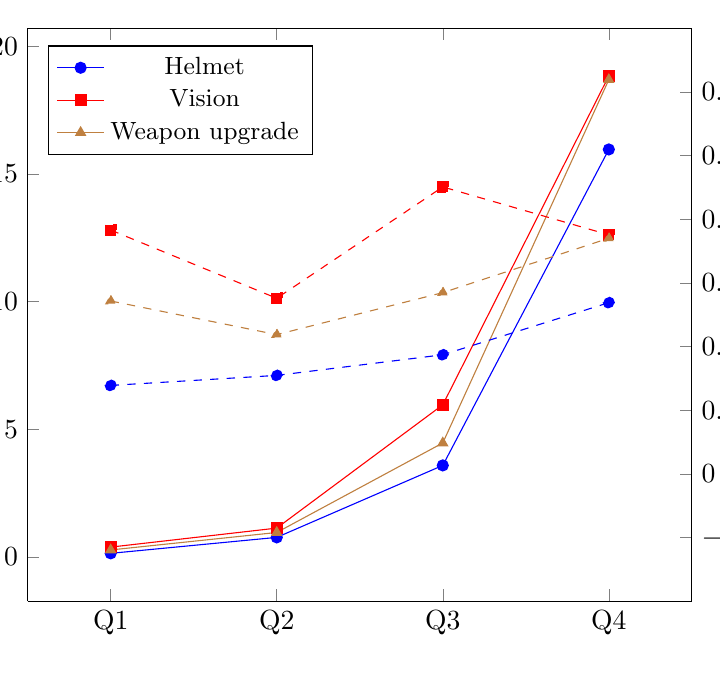
\begin{tikzpicture}[trim axis left, trim axis right]
    \pgfplotsset{set layers}
    \begin{axis}[ % avg
        scale only axis,
        ylabel=Avg. Price (solid),
        axis y line*=left,
        xmin=0.5, xmax=4.5,
        xtick=data,
        xticklabel={Q\pgfmathprintnumber{\tick}},
        legend entries={Helmet, Vision, Weapon upgrade},
        legend pos=north west,
        legend style={font=\small},
    ]
        \addplot[blue, mark=*] % Helmet
        coordinates {
            (1, 0.13879535558780817)
            (2, 0.763686440677965)
            (3, 3.582771084337348)
            (4, 15.957999999999998)
        };
        \addplot[red, mark=square*] % Vision
        coordinates {
            (1, 0.38291139240506333)
            (2, 1.1272)
            (3, 5.956296296296297)
            (4, 18.836363636363632)
        };
        \addplot[brown, mark=triangle*] % Weapon upgrade
        coordinates {
            (1, 0.27151898734177216)
            (2, 0.9558974358974357)
            (3, 4.461590909090908)
            (4, 18.690909090909088)
        };
    \end{axis}

    \begin{axis}[ % equiv
        scale only axis,
        axis x line=none,
        axis y line*=right,
        xmin=0.5, xmax=4.5,
        ymin=-0.2, ymax=0.7,
        ytick={-0.1, 0, 0.1, 0.2, 0.3, 0.4, 0.5, 0.6},
        ylabel=Equiv. Q1 Price (dashed)
    ]
        \addplot[dashed, blue, mark=*] % Helmet
        coordinates {
            (1, 0.13879535558780817)
            (2, 0.154562146892655)
            (3, 0.18697456492637202)
            (4, 0.2688148148148148)
        };
        \addplot[dashed, red, mark=square*] % Vision
        coordinates {
            (1, 0.38291139240506333)
            (2, 0.27573333333333333)
            (3, 0.4506995884773663)
            (4, 0.37542087542087527)
        };
        \addplot[dashed, brown, mark=triangle*] % Weapon upgrade
        coordinates {
            (1, 0.27151898734177216)
            (2, 0.21863247863247856)
            (3, 0.28462121212121194)
            (4, 0.37003367003366994)
        };
    \end{axis}
\end{tikzpicture}

        \caption{The average price of material equipments}\label{fig:reg_price_quality}
    \end{figure}

    As the dashed lines shown, we have many increasing segments, which means the aforementioned inequaly does not hold.
    This suggests our first strategy: For each $i$ where $P'_{i+1} > P'_i$, we can buy 3 Qi, then merge and sell an
    Qi\verb!+!1. For example, the most steep segment is Q2-Q3 Vision, we can profit from it by:
    \begin{enumerate}[nosep]
        \item buying 3 Q2 Vision at average price 1.127g;
        \item merging them with 1g fee to get an Q3 Vision;
        \item selling the Q3 Vision at average price 5.956g;
        \item the profit is $5.956 * 0.98 - (3 * 1.127 + 1) = 1.456$g.
    \end{enumerate}
    Such an easy strategy can achieve about 33\% profit rate, Wow!

    \subsection{Price distribution}

    The price of the a trade is a random variable, of course. We want to know the distribution $f_{q, s, p_1, p_2, t}(p)$ so
    we can appraise an equipment more precisely. The factors are 1) $q$: the quality, 2) $s$: the slot, 3) $p_1$, $p_2$:
    the two parameters, and 4) t: the time of a day when the trade ends. The $t$ is important because E-Sim is a global
    game, but most players live in the Europe. Given the design of the acution UI, players tends to bid when auctions are
    about to end. As a result, auctions that ends when European are sleeping are likely to sell in a lower price.

    Since the products' parameters are independent with the materials in merging and splitting, the price of materials
    should not depend on their parameters. We can first study the distribution of materials' prices.

    \begin{figure}[ht]
        \centering
        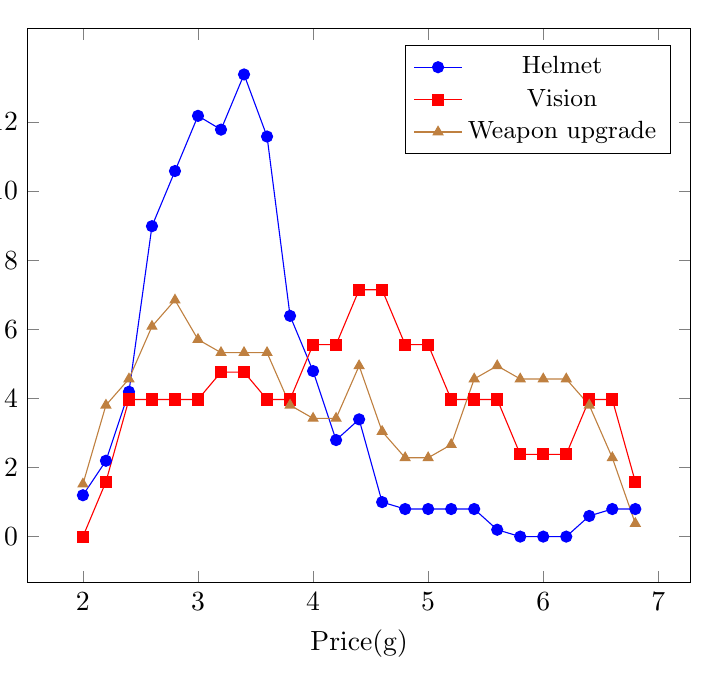
\begin{tikzpicture}[trim axis left, trim axis right]
    \begin{axis}[
        xlabel=Price(g),
        ylabel=Frequency(\%),
        ytick={0, 2, 4, 6, 8, 10, 12},
        legend entries={Helmet, Vision, Weapon upgrade},
        legend pos=north east,
        legend style={font=\small},
        width=10cm
    ]
        \addplot[blue, mark=*] % Helmet
        coordinates {
            (2.0, 1.197)
            (2.2, 2.195)
            (2.4, 4.191)
            (2.6, 8.982)
            (2.8, 10.578)
            (3.0, 12.175)
            (3.2, 11.776)
            (3.4, 13.373)
            (3.6, 11.576)
            (3.8, 6.387)
            (4.0, 4.790)
            (4.2, 2.794)
            (4.4, 3.393)
            (4.6, 0.998)
            (4.8, 0.798)
            (5.0, 0.798)
            (5.2, 0.798)
            (5.4, 0.798)
            (5.6, 0.199)
            (5.8, 0.000)
            (6.0, 0.000)
            (6.2, 0.000)
            (6.4, 0.598)
            (6.6, 0.798)
            (6.8, 0.798)
        };
        \addplot[red, mark=square*] % Vision
        coordinates {
            (2.0, 0.000)
            (2.2, 1.587)
            (2.4, 3.968)
            (2.6, 3.968)
            (2.8, 3.968)
            (3.0, 3.968)
            (3.2, 4.761)
            (3.4, 4.761)
            (3.6, 3.968)
            (3.8, 3.968)
            (4.0, 5.555)
            (4.2, 5.555)
            (4.4, 7.142)
            (4.6, 7.142)
            (4.8, 5.555)
            (5.0, 5.555)
            (5.2, 3.968)
            (5.4, 3.968)
            (5.6, 3.968)
            (5.8, 2.380)
            (6.0, 2.380)
            (6.2, 2.380)
            (6.4, 3.968)
            (6.6, 3.968)
            (6.8, 1.587)
        };
        \addplot[brown, mark=triangle*] % Weapon upgrade
        coordinates {
            (2.0, 1.520)
            (2.2, 3.802)
            (2.4, 4.562)
            (2.6, 6.083)
            (2.8, 6.844)
            (3.0, 5.703)
            (3.2, 5.323)
            (3.4, 5.323)
            (3.6, 5.323)
            (3.8, 3.802)
            (4.0, 3.422)
            (4.2, 3.422)
            (4.4, 4.942)
            (4.6, 3.041)
            (4.8, 2.281)
            (5.0, 2.281)
            (5.2, 2.661)
            (5.4, 4.562)
            (5.6, 4.942)
            (5.8, 4.562)
            (6.0, 4.562)
            (6.2, 4.562)
            (6.4, 3.802)
            (6.6, 2.281)
            (6.8, 0.380)
        };
    \end{axis}
\end{tikzpicture}

        \caption{The prices of different Q3 equipments}\label{fig:hist_material_price}
    \end{figure}

    Ummm, We have too few data to fit a usful model, so give up, for now.
\end{document}
